While the theory and phenomenology of exclusive processes and GPDs are now
rather mature, the extraction of GPDs (Compton form factors) from available
data is a complex problem that was started to be tackled only recently
\cite{Guidal:2008ie,Kumericki:2007sa,Moutarde:2009fg,Guidal:2009aa,
Guidal:2010ig,Guidal:2010de,Moutarde:2010uk,Moutarde:2011zz,Kumericki:2011aa}.
The complications include (i) generally low rates of exclusive processes, (ii)
the limited number of independent experimental observables which are measured,
(iii) the number of proton GPDs (at leading twist, the proton has four quark
and four gluon parton-helicity-conserving GPDs) which (iv) are themselves
functions of four variables, and (v) the fact that even at the leading order,
GPDs enter experimental observables in the form of convolutions with known
kernels. These convolutions are called Compton form factors (CFFs). There are
eight CFFs associated with the four quark helicity-conserving GPDs, namely
$Re\{\mathcal{H}\}$, $Re\{\mathcal{E}\}$, $Re\{\tilde{\mathcal{H}}\}$,
$Re\{\tilde{\mathcal{E}}\}$, $Im\{\mathcal{H}\}$, $Im\{\mathcal{E}\}$,
$Im\{\tilde{\mathcal{H}}\}$, and $Im\{\tilde{\mathcal{E}}\}$.

A quasi model-independent CFF fitting procedure of
Refs.~\cite{Guidal:2008ie,Guidal:2009aa,Guidal:2010ig,Guidal:2010de}
has been implemented for the TCS process. The procedure simultaneously fits
various experimental observables at a given kinematical point (\textit{i.e.},
$\eta$, $|t|$, and $Q^{\prime 2}$ for the TCS process), to the well-known
leading-twist and leading-order TCS and BH amplitude,

\begin{figure}[t]
\begin{center}
\mbox{
\subfigure{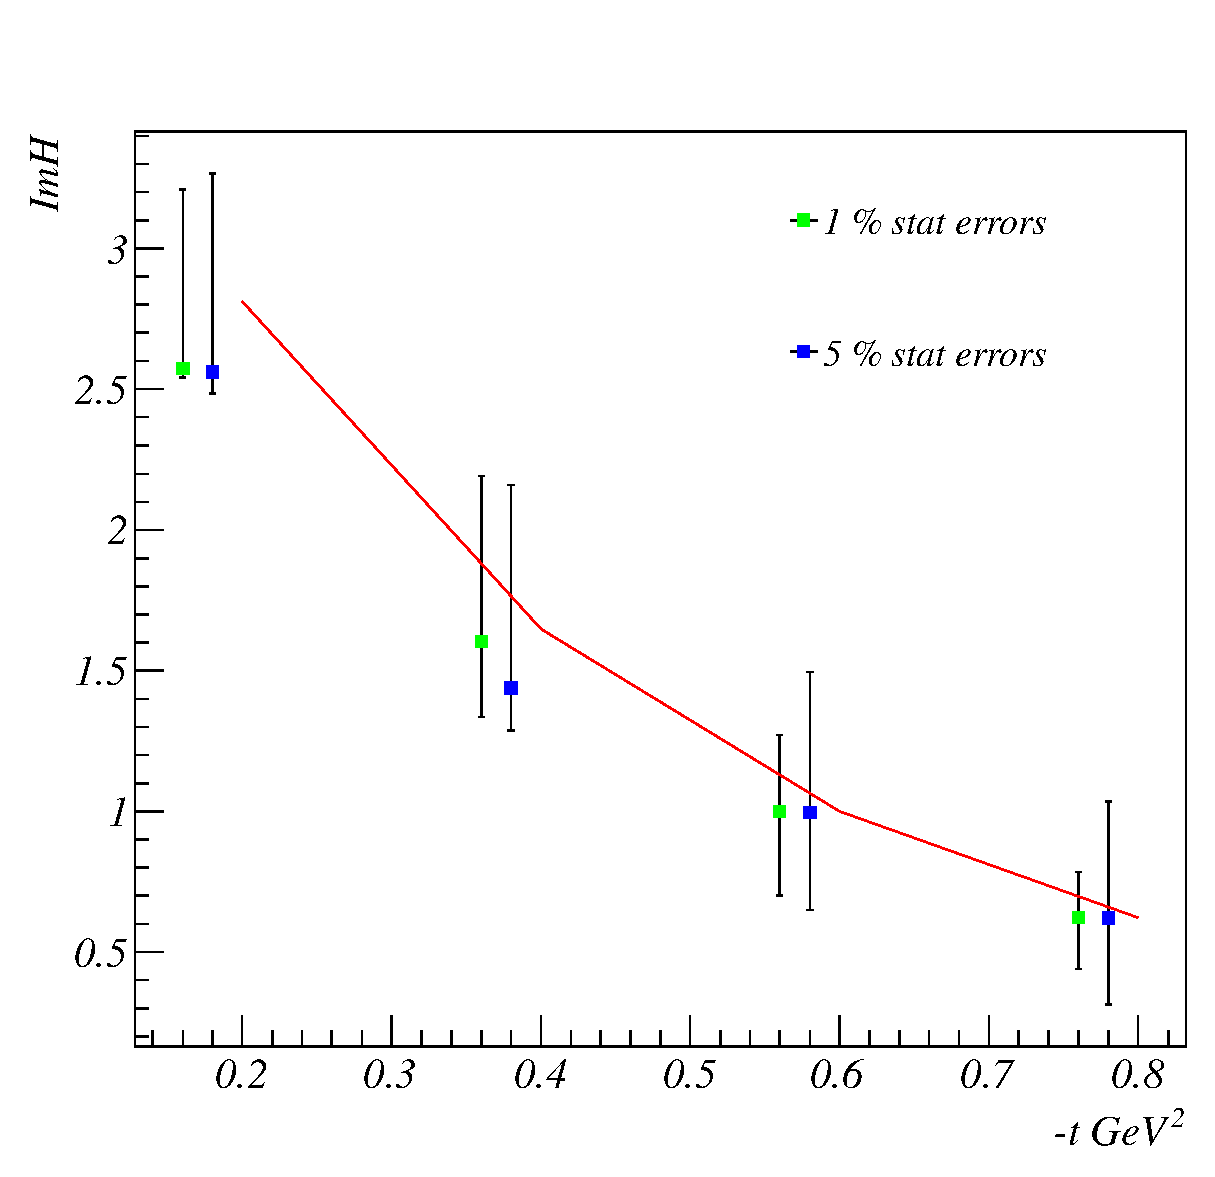
\includegraphics[scale=0.35]{ImH_theta.eps}} \quad
\subfigure{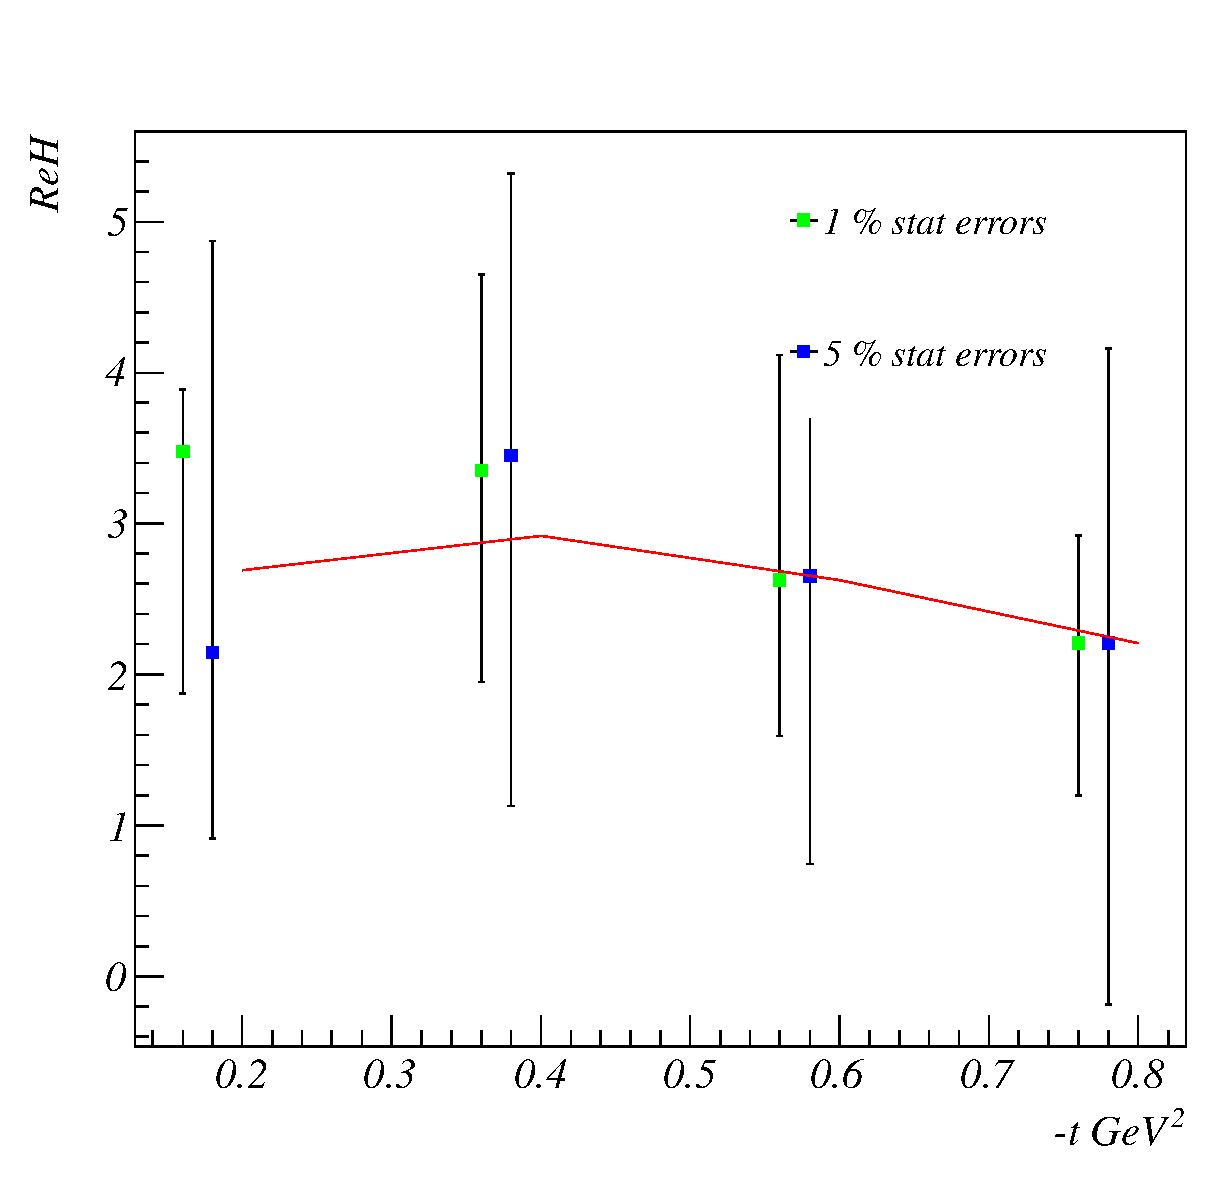
\includegraphics[scale=0.35]{ReH_theta.eps}}}
\end{center}
\caption{\small{
{\it Left panel:} result on the extraction of the $Im\{\mathcal{H}\}$ CFF 
for $E_e$=11 GeV, $Q'^2$=4 GeV$^2$ and $-t$=0.2, 0.4, 0.6 and 0.8 GeV$^2$.
{\it Right panel:} same for $Re\{\mathcal{H}\}$.
Symbols and curves are described in the text.}}
\label{fig:TCS_fits}
\end{figure}

This approach has been very successful for the DVCS process, allowing to
extract, at the $\approx$ 30\% level, from various beam- or target-polarized
observables, three CFFs
($Re\{\mathcal{H}\}$, $Im\{\mathcal{H}\}$, and $Im\{\tilde{\mathcal{H}}\}$)
in JLab and HERMES kinematics~\cite{Guidal:2010de}.
For this procedure to be efficient, it is important to simultaneously fit
several experimental observables. Fitting eight CFFs with only one observable
makes the problem too under-constrained.

To illustrate the quasi model-independent approach, we have generated
pseudo-data in typical 12 GeV kinematics ($E_e$=11 GeV, $Q'^2$=4 GeV$^2$,
and $|t|$=0.2, 0.4, 0.6, and 0.8 GeV$^2$), for two TCS observables that
we plan to extract: the unpolarized cross section and the polarized beam
asymmetry. The CFFs used for the generation of the data were the
VGG~\cite{Vanderhaeghen:1999xj,Guidal:2004nd} ones. Assuming different values
for the experimental uncertainties on these two observables, we then fitted
them and attempted to recover the generated CFFs. The results of the fit
revealed a sensitivity to four CFFs:
$Re\{\mathcal{H}\}$, $Im\{\mathcal{H}\}$, $Re\{\tilde{\mathcal{H}}\}$, and
$Im\{\tilde{\mathcal{H}}\}$. Fig.~\ref{fig:TCS_fits} shows our result for
$Re\{\mathcal{H}\}$ and $Im\{\mathcal{H}\}$, which are the most constrained.
The red curve shows the generated CFFs, while the blue and green points show
the resulting fitted CFFs with their associated error bar, corresponding to
a 5\% and a 1\% uncertainty, respectively, on the experimental cross section
and asymmetry. Due to systematics, a 1\% uncertainty on the experimental
observable will probably always be unrealistic, but we nevertheless show
the result for reference.
Fig.~\ref{fig:TCS_fits} shows that with a 5\% total experimental uncertainty,
we should be able to extract the $Re\{\mathcal{H}\}$ and $Im\{\mathcal{H}\}$
CFFs with $\approx$ 60\% and 20\% error, respectively.
The resulting errors may appear large, but we stress that firstly, this
fitting method aims to be model-independent, and secondly, that in this
procedure, the error on the extracted CFFs is not directly proportional to the
precision of the experimental data but rather reflects the influence (or our
ignorance) of all the other CFFs. The sub-dominant (kinematically suppressed)
CFFs enter the fitting procedure and have an impact on the error.
Therefore, the errors on $Re\{\mathcal{H}\}$ and $Im\{\mathcal{H}\}$ in
Fig.~\ref{fig:TCS_fits} reflect the ``correlation'' between all eight CFFs.
Increasing the number of experimental observables to be fitted (for instance,
using a longitudinally and/or a transversely polarized target) will strongly
reduce the fitting errors, and the uncertainties on the extracted CFFs will
more directly reflect the precision of the data. Alternatively, model
constraints can be added to achieve a similar result with only two
observables. Either way, ultimately data with small uncertainties, both
statistical and systematic, will have a large impact on our understanding of
the CFFs. But the initial results presented in Fig.~\ref{fig:TCS_fits} already
demonstrate the general feasibility of extraction of GPDs from TCS data.
